\chapter{Introduction ultracold atomc systems}
\label{ch:qs}

This chapter intends to provide a simple introduction to fundamental quantum concepts used for simulations throughout this body of work.

\section{The Schr\"odinger equation and the Hamiltonian}
Quantum particles are often described by their wavefunction, $\Psi(\mathbf{r},t)$, where $\mathbf{r}$ is a position-space variable and $t$ is time.
This does not have a simple physical interpretation; however, the wavefunction density, $|\Psi(\mathbf{r},t)|^2$, can be interpreted as a probability distribution in position-space, where peaks represent areas where quantum particles are likely to be found.
As with most probability distributions,

\begin{equation}
    \label{eqn:norm}
    \int_\infty^\infty |\Psi(\mathbf{r},r)|^2 d\mathbf{r} = N,
\end{equation}

\noindent where $N$ is the number of particles in the system.
For certain simulations with the SSFM method, it is important to ensure the quantum system is normalized correctly and Equation~(\ref{eqn:norm}) is used for this purpose.
This will be discussed in further detail in Chapter~\ref{ch:splitop}.

For the purposes of this body of work, we can simulate the dynamics of a quantum system by solving the Schr\"odinger equation,

\begin{equation}
    i\hbar\frac{\partial\Psi(\mathbf{r},t)}{\partial t} = \left(\frac{p^2}{2m} + V_0\right) \Psi(\mathbf{r},t)
    \label{eqn:schrody}
\end{equation}

\noindent where $m$ is the mass of the atomic system, $p = -i\hbar\nabla$ is the momentum operator, and $V_0$ is the trapping potential.
This is a partial differential equation that relates the change in the wavefunction with time on the left-hand side to physical arguments like momentum and position on the right.
For this reason, the operators on the right-hand side are often described as the \textit{Hamiltonian operator}, 

\begin{equation}
\mathcal{\hat H} = \frac{p^2}{2m} + V_0
\end{equation}

\noindent which noticeably has two separate operators: one in momentum-space ($\mathcal{\hat H}_p = \frac{p^2}{2m}$) and another in position-space ($\mathcal{\hat H}_v = V_0$).
The Hamiltonian describes how the quantum system evolves with time, and in this work, we modify the Hamiltonian to match the various quantum systems we would like to simulate.

\begin{figure}

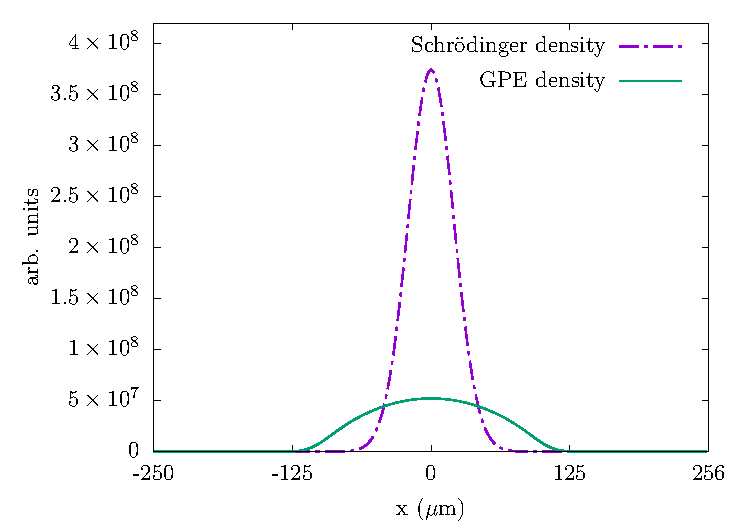
\includegraphics[width = \textwidth]{data/qs/SHO/SHO.pdf}

\caption{Simulated results from ground-state evolution from the split-step Fourier method after 10,000 steps. Here, we use a Rubidium 87 atom with $\omega_x = 1$Hz on a 256-point grid of size 200 $\mu$m. The wavefunction has been normalized such that $\int_{-\infty}^\infty|\Psi|^2 dx = 1$, which provides arbitrary units. We have scaled the potential by $m \omega_x^2 dx^2$ to match these units. This simulation was performed with the GPUE codebase \cite{schloss2018}.}
\label{fig:SHO}
\end{figure}

When the quantum system is in its lowest energy state, the probability distribution will often follow the trapping potential.
For example, in the case of the simple harmonic oscillator in one dimension, $V_0 = m \omega_x x^2$, where $\omega_x$ is the trapping frequency in the $x$-dimension and describes the tightness of the trap.
Figure~\ref{fig:SHO} shows the lowest energy state, also called the \textit{ground state} of a quantum system consisting of a single particle.
Notably, the quantum particle rests in the center of the trap and if the trap is moved, the particle will move with it and oscillate about the new trap location.
Many quantum engineering systems require precise control of the trapping potential to manipulate quantum systems~\cite{menchon2016}, and we will discuss two such methods (quantum optimal control~\cite{werschnik2007} and shortcuts to adiabaticity~\cite{guery2019}) in Chapter~\ref{ch:1d}.

Quantum systems do now always have a straightforward interpretation, and $\Psi(\mathbf{r},t)$ is a complex-valued object with operators in both position and momentum space.
As such, it is important to discuss fundamental relationships between position and momentum space in order to better understand quantum systems, and ultimately how the SSFM acts in both spaces.

\section{The Heisenberg uncertainty principle}

\jrs{NC; Maybe move this to the splitop chapter, as well?}

The Heisenberg uncertainty principle is a relation between the position and momentum components of a quantum system.
This principle simply states that

$$
\sigma_x \sigma_p \geq \frac{\hbar}{2},
$$

where $\sigma_x$ and $\sigma_p$ are the standard deviations of the position-space and momentum-space distributions for a quantum system.
Because these two variables are inversely proportional, this can be interpreted to mean that as the measurement in one domain becomes more precise, the measurement in to conjugate domain becomes less so.
This is historically interesting, as it seems to provide a fundamental limit to the precision by which the momentum or position of a quantum particle is known.

For the purposes of this work, we do not need to delve too deeply into the interpretation of this principle.
Instead, we need to find an appropriate mathematical formalism that allows for us to easily recreate the same properties, and thus develop a method for transforming between position and momentum space for quantum simulations.
In this case, we can see this relation simply by performing a Fourier transform on a set of gaussians with an increasing standard deviation, as shown in FIGURE -- SHOW ~10 INCREASINGLY THICK GAUSSIANS NEXT TO THEIR FOURIER TRANSFORM, K
EEPING THE COLORS CONSISTENT.

As such, it is worth exploring the Fourier transform, itself, and discussing its various applications.
Further discussions about numerical methods for implementing the Fourier transform will be discussed in Chapter~\ref{ch:splitop}.

\section{The Fourier transform}

\jrs{CN}

The Fourier transform is a fundamental mathematical technique that lies at the heart of signal processing.
Because it is such a fundamental technique, there are many intuitive descriptions for interpreting the Fourier transform, and it would not be worthwhile to discuss all of these explanations here.
In most cases, the Foureir transform is introduced as a transformation between the time domain and frequency domain.
If we have some wave in the time domain with some frequency $\omega$, such as $\sin(2\pi\omega)$, we can plot the signal fully in the time-domain; however, the signal changes to a single peak in the frequency domain, as shown in Figure [ADD](a).

In fact, every point in the frequency domain corresponds to another distinct wave in the time-domain.
As such, we can decompose most wave-like signals into a sparse set of delta-like peaks in the frequency domain, and this can be seen in Figure [ADD].
This sparsity has been used for many applications, including compressed sensing, which allows us to reconstruct high-resolution data from low-resolution ouput in a separate domain~\cite{baraniuk2011}.
We will discuss this in more depth in Chapter~\ref{ch:splitop} when we discuss the compressed split-step Fourier method, which applies tecniques in compressive sensing to the SSFM \cite{bayindir2015}.

Mathematically, the Fourier transform can be represented as,

$$
\mathcal{F}(\xi) = \int_{-\infty}^{\infty}f(t)e^{-2\pi i t \xi}dt
$$

\noindent and the inverse Fourier transform can be represented as,

$$
f(t) = \int_{-\infty}^{\infty}\mathcal{F}(\xi)e^{2\pi i t \xi}d\xi
$$

\noindent where $t$ is an element in the time-domain, $\xi$ is an element in the frequency domain, $f(t)$ is a time-domain function, and $\mathcal{F}(\xi)$ is a corresponding frequency-domain function.
In almost all cases related to this work, it is equally important to discuss the Discrete Fourier Transform (DFT), for which the forward transform is,

$$
X_k = \sum_{n=0}^{N-1} x_n e^{-2 \pi i k n / N}
$$

\noindent and the inverse transform is,

$$
x_n = \frac{1}{N} \sum_{k=0}^{N-1} X_k e^{2 \pi i k n / N}
$$

\noindent where $X_k$ and $x_n$ represent the frequency and time domain signals, respectively, $k$ is a component in the frequency domain, $x$ is a component in the time domain, and N is the total number of elements in the signal.
Though the primary difference between these two definitions is that the DFT replaced the integral of the Fourier transform with a sum, the DFT also allows for the computational investigation of signal processing, as it can now be interpreted as a sum and matrix multiplication.
ADD DISCUSSION ON DFT MATRIX? PROBABLY NOT RELEVANT...
Unfortunately, this comes at a huge cost for complexity, as the matrix multiplication, alone, is of the order of $\mathcal{O}(n^3)$, and with the sum, the DFT has a heafty computational complexity of $\mathcal{O}(n^4)$, assuming a square signal.

Luckily, there have been several successful attempts to create a Fast Fourier Transform (FFT), including the Cooley-Tukey method, that was first discovered by Gauss and then later contemporized by Cooley and Tukey when they independently discovered it \cite{cooley1965}.
This method is not straightforwardly parallelizable; however, it has become so fundamental to signal processing, that it has become incredibly well-optimized with several libraries, including FFTW~\cite{frigo1998} and CuFFT~\cite{fatica2008} for distributed and GPU calculations, respectively.

We will discuss the Cooley-Tukey method, itself, along with different parallelization methods for multi-GPU simulations in Chapter~\ref{ch:splitop}.
For now, we will turn our focus to attributes of the physical systems we will be simulating throughout this work, ultracold atoms.

\section{Introduction to ultracold quantum systems}

As atomic systems are cooled to temperatures near absolute zero Kelvin, it becomes easier to discern their quantum properties which vary depending on the system.
Most elementary particles that make up atoms have intrinsic angular momentum known as \textit{spin}.
Electrons are elementary particles with a spin of $\frac{1}{2}$, and protons and nuetrons are made of elementary particles that sum to a spin of $\frac{1}{2}$.
The spin of the entire atom is determined by summing the constituent spin components.
If the sum results in an integer value, the atom is known as a \textit{boson}, and if the sum results in a half-integer value, the atom is known as a \textit{fermion}.

Because fermions have half-integer spin, they must obey the Pauli exclusion principle and are constrained to Fermi--Dirac statistics, which means their ground state will be composed of several fermionic pairs.
This creates a \textit{Fermi sea}, where particles fill defined energy levels from the bottom up with two particles per level.

On the other hand, bosons have integer spin and follow Bose--Einstein statistics and will condense into a single, macroscopic ground state when cooled~\cite{Einstein1925, Fetter2003}.
This state of matter is known as a Bose--Einstein Condensate (BEC) and it has the properties of a superfluid, this will be discussed fully in Chapter~\ref{ch:vortex}.

There are notable exceptions to these rules, such as the highly correlated Tonks--Girardeau gas where bosons may act as spinless, non-interacting fermions \cite{Girardeau}.
There also exists a regime where interacting fermions can also condense into a BEC-like system~\cite{Nozieres1985, Bulgac2014}, but this work focuses primarily on bosonic systems and will not discuss fermionic systems further.
Now we will extend this framework to two important quantum systems: the Bose--Einstein condensate and the Tonks--Girardeau gas, both of which are used heavily in this work.

\subsection{Bose--Einstein condensation and the Gross--Pitaevskii Equation}

As mentioned in Section~\ref{sec:introintro}, bosons in a BEC condense into the same (ground) state, meaning we must introduce a many-body Hamiltonian for the system and take inter-particle interactions into account.
For the purposes of this body of work, we will only consider two-body interactions and assume any interactions between three or more atoms are unlikely and negligible.
We may write the Hamiltonian with two body interactions in the second quantized form as
\begin{equation}
    \hat H = \int d\mathbf{r} \hat \Psi^\dagger(\mathbf{r})\left[-\frac{\hbar^2}{2m}\nabla^2 + V_0(\mathbf{r}) \right]\hat \Psi(\mathbf{r}) + \frac{1}{2} \int d\mathbf{r} d\mathbf{r'} \hat \Psi^\dagger(\mathbf{r}) \hat \Psi^\dagger(\mathbf{r'}) V(\mathbf{r} - \mathbf{r'})\hat \Psi(\mathbf{r'}) \hat \Psi(\mathbf{r})
    \label{eqn:2nd}
\end{equation}
where $\mathbf{r}$ and $\mathbf{r'}$ are the positions of the two colliding particles, $V(\mathbf{r}-\mathbf{r'})$ is the interaction potential, and $\hat \Psi^\dagger(\mathbf{r})$ and $\hat \Psi(\mathbf{r})$ are the creation and annihilation operators that follow the commutation relation, $[\hat \Psi(\mathbf{r}),\hat \Psi^\dagger(\mathbf{r})] = \delta(\mathbf{r} - \mathbf{r'})$.

In the case of a BEC at $T\approx0$, we may perform a Bogoliubov expansion~\cite{Bogoliubov1947, Dalfovo1999}
\begin{equation}
    \hat \Psi (\mathbf{r}, t) = \Phi(\mathbf{r},t) + \delta \hat \Phi(\mathbf{r},t)
\label{eqn:bog}
\end{equation}
where $\Phi(\mathbf{r},t) \equiv \langle \hat \Psi(\mathbf{r},t) \rangle$ is the wavefunction of the condensate known as the ``order parameter'' and $\delta \hat \Phi(\mathbf{r},t)$ represents fluctuations of the BEC system.
In a BEC, the condensate density is defined as
\begin{equation}
    n(\mathbf{r},t) = |\Phi(\mathbf{r},t)|^2.
\end{equation}

Now we may use the Heisenberg equation of motion
\begin{equation}
    i\hbar \frac{\partial}{\partial t}\hat \Psi(\mathbf{r},t) = [\hat \Psi, \hat H]
\end{equation}
    to determine the time evolution of the field operator $\hat \Psi(\mathbf{r},t)$ as
\begin{equation}
    \frac{\partial}{\partial t}\hat \Psi(\mathbf{r},t) = \frac{1}{i\hbar}\left[-\frac{\hbar^2}{2m}\nabla^2 + V_0(\mathbf{r}) + \int d\mathbf{r'} \hat \Psi^\dagger(\mathbf{r'}, t)V(\mathbf{r'} -\mathbf{r})\hat \Psi(\mathbf{r'},t)\right]\hat \Psi(\mathbf{r},t),
\end{equation}
which follows from Equation~\eqref{eqn:2nd} after integrating over $\mathbf{r}$. 
Now we must apply a few approximations for the BEC:
\begin{enumerate}
    \item In the Bogoliubov expansion, Equation~\eqref{eqn:bog}, we assume that $\delta \hat \Phi(\mathbf{r},t)$ is small at $T = 0\text{K}$, and thus $\hat \Psi(\mathbf{r},t) \approx \Phi(\mathbf{r},t)$. 
    \item Two bosons will only interact with a contact potential of the form
    \begin{equation}
        V(\mathbf{r'}-\mathbf{r}) = g\delta(\mathbf{r'} - \mathbf{r}),
    \end{equation}
    which has a strength given by
    \begin{equation}
        g \equiv \frac{4 \pi \hbar^2 a_s}{m},
    \end{equation}
    where $a_s$ is the species and state-dependent s-wave scattering length.
    %\item The bose gas is dilute and the inter-particle spacing is much larger than $a_s$.
\end{enumerate}

With these approximations, we may write the time-dependent Schr\"odinger equation as
\begin{equation}
    i\hbar \frac{\partial}{\partial t}\Phi(\mathbf{r},t) = \left( - \frac{\hbar^2}{2m} \nabla^2 + V_0(\mathbf{r}) + g |\Phi(\mathbf{r},t)|^2\right)\Phi(\mathbf{r},t).
\end{equation}
This equation is known as the nonlinear Schr\"odinger equation due to the presence of the $|\Phi(\mathbf{r},t)|^2$ term.
In the BEC community, the equation is usually called the Gross-Pitaevskii equation (GPE).
When written in the time-independent form it determines the chemical potential $\mu$ of the condensate system~\cite{Gross1961, Pitaevskii1961}
\begin{equation}
    \mu\Phi(\mathbf{r}) = \left( - \frac{\hbar^2}{2m} \nabla^2 + V_0(\mathbf{r}) + g |\Phi(\mathbf{r})|^2\right)\Phi(\mathbf{r},t).
    \label{eqn:GP}
\end{equation}

This equation allows us to determine the full dynamics of a BEC system and the numerical solutions will be discuss in Section~\ref{sec:code}. Similar derivations of the GPE can be found in many introductory texts on BEC physics, such as~\cite{Fetter2003,  Pethick2002, Fetter2009}.

\subsection{Tonks--Girardeau gas}

As discussed, the Tonks--Girardeau gas consists of a number of bosons that have the properties of spinless, non-interacting fermions.
This is a particular case of the one-dimensional GPE where $g\rightarrow\infty$.
In this case, the bosons cannot pass each other and cannot be at the same location, which acts formally similar to the Pauli-exclusion principle for fermionic sstems.
In this case, the Hamiltonian can be solved by the Bose--Fermi mapping theorem \cite{girardeau2001ground, girardeau2001measurement}, which replaces the interaction terms in the hamiltonian with a boundary condition on the many-body bosonic wavefunction.

\begin{equation}
\Psi_B(x_1, x_2, \ldots, x_N) = 0,\qquad \mathrm{if}\qquad x_i - x_j = 0 \quad\textrm{with}\quad i \ne j.
\end{equation}

The Bose--Fermi mapping theorem allows us to replace strongly interacting bosons by spinless, non-interacting fermions, on which we can use the Slater determinant \jrs{CN},

\begin{equation}
\Psi_F (x_1, x_2, \ldots, x_N) = \frac{1}{\sqrt{N}} \det\Big[\psi_n(x_j)\Big]_{n,j=1}^N.
\end{equation}

\noindent where $\psi_n(x_j)$ are the single-particle eigenstates of the trapping potential $V_0$.
Because the Fermionic many-body wavefunction is antisymmetric, this needs to be symmetrerized for bosonic states as, 

\begin{equation}
\Psi_B(x_1, x_2, \ldots, x_N) =
\prod_{i < j}
\mathrm{sgn}(x_i - x_j)\Psi_F(x_1, x_2, \ldots, x_N)
\end{equation}

\noindent which means that calculating the time evolution of a Tonks--Girardeau gas requires evolving single-particle states, governed by a simple Hamiltonian.
